%First Beamer Talk

\documentclass{beamer}

% Setup appearance:

\usetheme{Darmstadt}
%\usecolortheme{lily}
%\usefonttheme[onlylarge]{structurebold}
%\setbeamerfont*{frametitle}{size=\normalsize,series=\bfseries}
%\useinnertheme{circles}


% Standard packages

\usepackage[english]{babel}
\usepackage[latin1]{inputenc}
%\usepackage{times}
\usepackage[T1]{fontenc}
\usepackage{multirow}
\usepackage{capt-of}
\usepackage{graphicx}
\usepackage{array}
\usepackage{tikz}

\setbeamertemplate{blocks}[rounded] [shadow=false]

% Some optional colors. Change or add as you see fit.
%---------------------------------------------------
 \definecolor{ualbertagreen}{HTML}{007C41}
\definecolor{ualbertagold}{HTML}{FFDB05}


% Some optional color adjustments to Beamer. Change as you see fit.
%------------------------------------------------------------------
\setbeamercolor{frametitle}{fg=ualbertagreen,bg=white}
\setbeamercolor{title}{fg=ualbertagreen,bg=white}
\setbeamercolor{author}{fg=ualbertagreen,bg=white}
\setbeamercolor{date}{fg=ualbertagreen,bg=white}
\setbeamercolor{affiliation}{fg=ualbertagreen,bg=white}
\setbeamercolor{institute}{fg=ualbertagreen,bg=white}
\setbeamercolor{local structure}{fg=ualbertagreen}
\setbeamercolor{section in toc}{fg=ualbertagreen,bg=white}
% \setbeamercolor{subsection in toc}{fg=ualbertagreen,bg=white}
\setbeamercolor{footline}{fg=ualbertagreen!50, bg=white}
\setbeamercolor{block title}{fg=ualbertagreen,bg=white}
\setbeamercolor{upper separation line head}{bg=ualbertagreen}
\setbeamercolor{lower separation line head}{bg=ualbertagold}
\setbeamercolor{middle separation line head}{bg=ualbertagold}
\setbeamercolor{frametitle}{fg=ualbertagreen,bg=white}

\setbeamercolor{section in head/foot}{bg=white,fg=ualbertagreen}
\setbeamercolor{author in head/foot}{bg=white,fg=ualbertagreen}
\setbeamercolor{date in head/foot}{bg=white,,fg=ualbertagreen}
\setbeamercolor{title in head/foot}{bg=white,fg=ualbertagreen}

\setbeamercolor{headline}{bg=white,fg=ualbertagreen}




\setbeamercolor{middle separation line head}{bg=ualbertagreen}
\setbeamercolor{alerted text}{fg=red}
\setbeamercolor{example text}{fg=black}
\setbeamercolor{structure}{fg=black}

% Various cosmetic things, though I must confess I forget what exactly these do and why I included them.
%-------------------------------------------------------------------------------------------------------
\setbeamercolor{structure}{fg=ualbertagreen}


\setbeamercolor{local structure}{parent=structure}
\setbeamercolor{item projected}{parent=item,use=item,fg=ualbertagreen,bg=white}
\setbeamercolor{enumerate item}{parent=item}

\setbeamertemplate{title page}{%
  \vbox{}
%  \vfill
    \vspace{0cm}% NEW
  \begingroup
    \centering
    \begin{beamercolorbox}[sep=8pt,center]{title}
      \usebeamerfont{title}\inserttitle\par%
      \ifx\insertsubtitle\@empty%
      \else%
        \vskip0.05em%
        {\usebeamerfont{subtitle}\usebeamercolor[fg]{subtitle}\insertsubtitle\par}%
      \fi%
    \end{beamercolorbox}%
    \vskip1em\par
    \begin{beamercolorbox}[sep=8pt,center]{author}
      \usebeamerfont{author}\insertauthor
    \end{beamercolorbox}
    \begin{beamercolorbox}[sep=8pt,center]{institute}
      \usebeamerfont{institute}\insertinstitute
    \end{beamercolorbox}
    \vspace{0.5cm}% NEW
    \begin{beamercolorbox}[sep=8pt,center]{date}
      \usebeamerfont{date}\insertdate
    \end{beamercolorbox}\vskip0.05em
%    {\usebeamercolor[fg]{titlegraphic}\inserttitlegraphic\par}
  \endgroup
%  \vfill
}


\logo{
   \tikz [remember picture,overlay]
    \node[yshift=.3cm,xshift=1.5cm] at (current page.south west)
        %or: (current page.center)
        {\includegraphics[width=1in]{UA-ASB-COLOUR.png}};
%\includegraphics[height=0.8cm]{UA-ASB-COLOUR.png}\vspace{220pt}
}




\setbeamertemplate{headline}{%
\leavevmode%
  \hbox{%
    \begin{beamercolorbox}[wd=\paperwidth,ht=5ex,dp=1.825ex]{white}%
    \usebeamerfont{headline}\hskip6pt\inserttitle\par%
    \insertsectionnavigationhorizontal{\paperwidth}{}{\hskip0pt plus1filll}
    \end{beamercolorbox}%
  }
}

\setbeamertemplate{sidebar right}{}


\logo{
   \tikz [remember picture,overlay]
    \node[yshift=.3cm,xshift=1.5cm] at (current page.south west)
        %or: (current page.center)
        {\includegraphics[width=1in]{UA-ASB-COLOUR.png}};
%\includegraphics[height=0.8cm]{UA-ASB-COLOUR.png}\vspace{220pt}
}




%\setbeamertemplate{footline}{%
%\hfill\usebeamertemplate***{navigation symbols}
%\hspace{1cm}\insertframenumber{}/\inserttotalframenumber}
\defbeamertemplate*{footline}{my footline}{%
    \ifnum\insertpagenumber=1
        \Tiny{%
            \hfill%
		\vspace*{1pt}%
            %\insertframenumber/\inserttotalframenumber \hspace*{0.1cm}%
            \newline%
            \color{ualbertagold}{\rule{\paperwidth}{0.4mm}}\newline%
            \color{ualbertagold}{\rule{\paperwidth}{.4mm}}%
        }
%    \hbox{%
%        \begin{beamercolorbox}[wd=\paperwidth,ht=.8ex,dp=1ex,center]{}%
%      % empty environment to raise height
%        \end{beamercolorbox}%
%    %}%
    %\vskip0pt%
    %no page number on the first page
    %    \Tiny{%
    %        \hfill%
   % 		\vspace*{1pt}%
    %        \color{ualbertagold}{\rule{\paperwidth}{0.4mm}}\newline%
    %        \color{ualbertagold}{\rule{\paperwidth}{.4mm}}%
%        }%
  \else%
        \Tiny{%
            \hfill%
		\vspace*{1pt}%
            \insertframenumber/\inserttotalframenumber \hspace*{0.1cm}%
            \newline%
            \color{ualbertagold}{\rule{\paperwidth}{0.4mm}}\newline%
            \color{ualbertagold}{\rule{\paperwidth}{.4mm}}%
        }%
    \fi%
}




\usepackage[style=british]{csquotes}

\def\signed #1{{\leavevmode\unskip\nobreak\hfil\penalty50\hskip1em
  \hbox{}\nobreak\hfill #1%
  \parfillskip=0pt \finalhyphendemerits=0 \endgraf}}

\newsavebox\mybox
\newenvironment{aquote}[1]
  {\savebox\mybox{#1}\begin{quote}}
  {\vspace*{1mm}\signed{\usebox\mybox}\end{quote}}






\renewcommand{\(}{\begin{columns}}
\renewcommand{\)}{\end{columns}}
\newcommand{\<}[1]{\begin{column}{#1}}
\renewcommand{\>}{\end{column}}
%%%%%%%%%%%%%%%%%%%%%%%%%%%%%%%%%%%%%%%%%%%%%%%%%%





% Author, Title, etc.

\title[Measuring the Impacts of Energy Infrastructure, Ottawa 2018]
{%
  Pipelines, netbacks and trade - the value of pipelines to the oil sands%
}

\author[Leach]
{
  Andrew~Leach
}

\institute[2018]
{
  Alberta School of Business, University of Alberta
 }

\date[10/18/2018]
{\today}


\newcommand{\degC}{$^o$C$\,$}
\newcommand{\co}{$\text{CO}_{2}\,$}
\newcommand{\tx}{$G_{2\times\text{CO}_2}$}
\newcommand{\Real}{\mathbb R}



% The main document


\begin{document}

\begin{frame}
   \tikz [remember picture,overlay]
    \node[yshift=-0.95cm,xshift=0cm] at (current page.north)
        %or: (current page.center)
        %\node[yshift=-0.75cm,xshift=4.5cm] at (current page.north west)
        %{\includegraphics[width=3in]{UA-ASB-COLOUR.png}};
        {\includegraphics[width=\paperwidth]{../../EE_logo.png}}; \vspace{1cm}
   \titlepage
   \vfill
\end{frame}



\section{Introduction}

\begin{frame}{Key Points}
\begin{itemize}
\setlength\itemsep{0 em}
\item Infrastructure is crucial for future oil sands viability, especially under low(er) prices;
\item Infrastructure demands in Canada have changed, as have prices and potential netbacks - the prize is not as big as it once was;
\item Policy changes (C-69, etc.) are not asking for the impossible on climate change tests - in fact, they're not really asking for much at all;
\end{itemize}
\vfill
\end{frame}



\section{Bitumen Netbacks}

\begin{frame}{What do we mean when we talk about netbacks?}
   \tikz [remember picture,overlay]
    \node[yshift=-.75cm,xshift=0cm] at (current page.center)
        {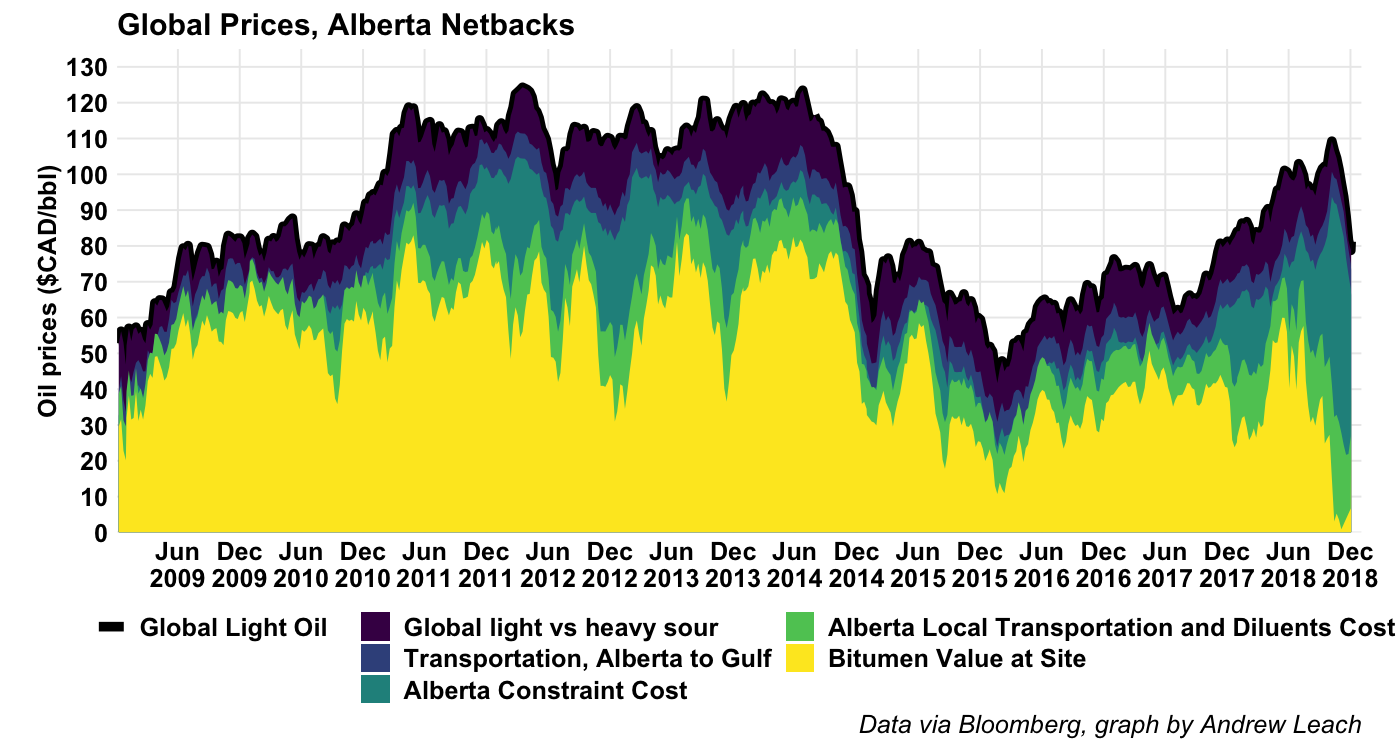
\includegraphics[width=.9\paperwidth]{cdn_bitumen_net.png}}; \vspace{1cm}
   \vfill
\end{frame}


\begin{frame}{Why is Alberta oil fetching low prices? Not enough pipeline capacity to meet demand}
   \tikz [remember picture,overlay]
    \node[yshift=-.75cm,xshift=0cm] at (current page.center)
        {\includegraphics[width=.9\paperwidth]{../../pipe_capacity_real.png}}; \vspace{1cm}
   \vfill
\end{frame}


\begin{frame}{Why is Alberta oil fetching low prices? Lower value crude}
   \tikz [remember picture,overlay]
    \node[yshift=-.75cm,xshift=0cm] at (current page.center)
        {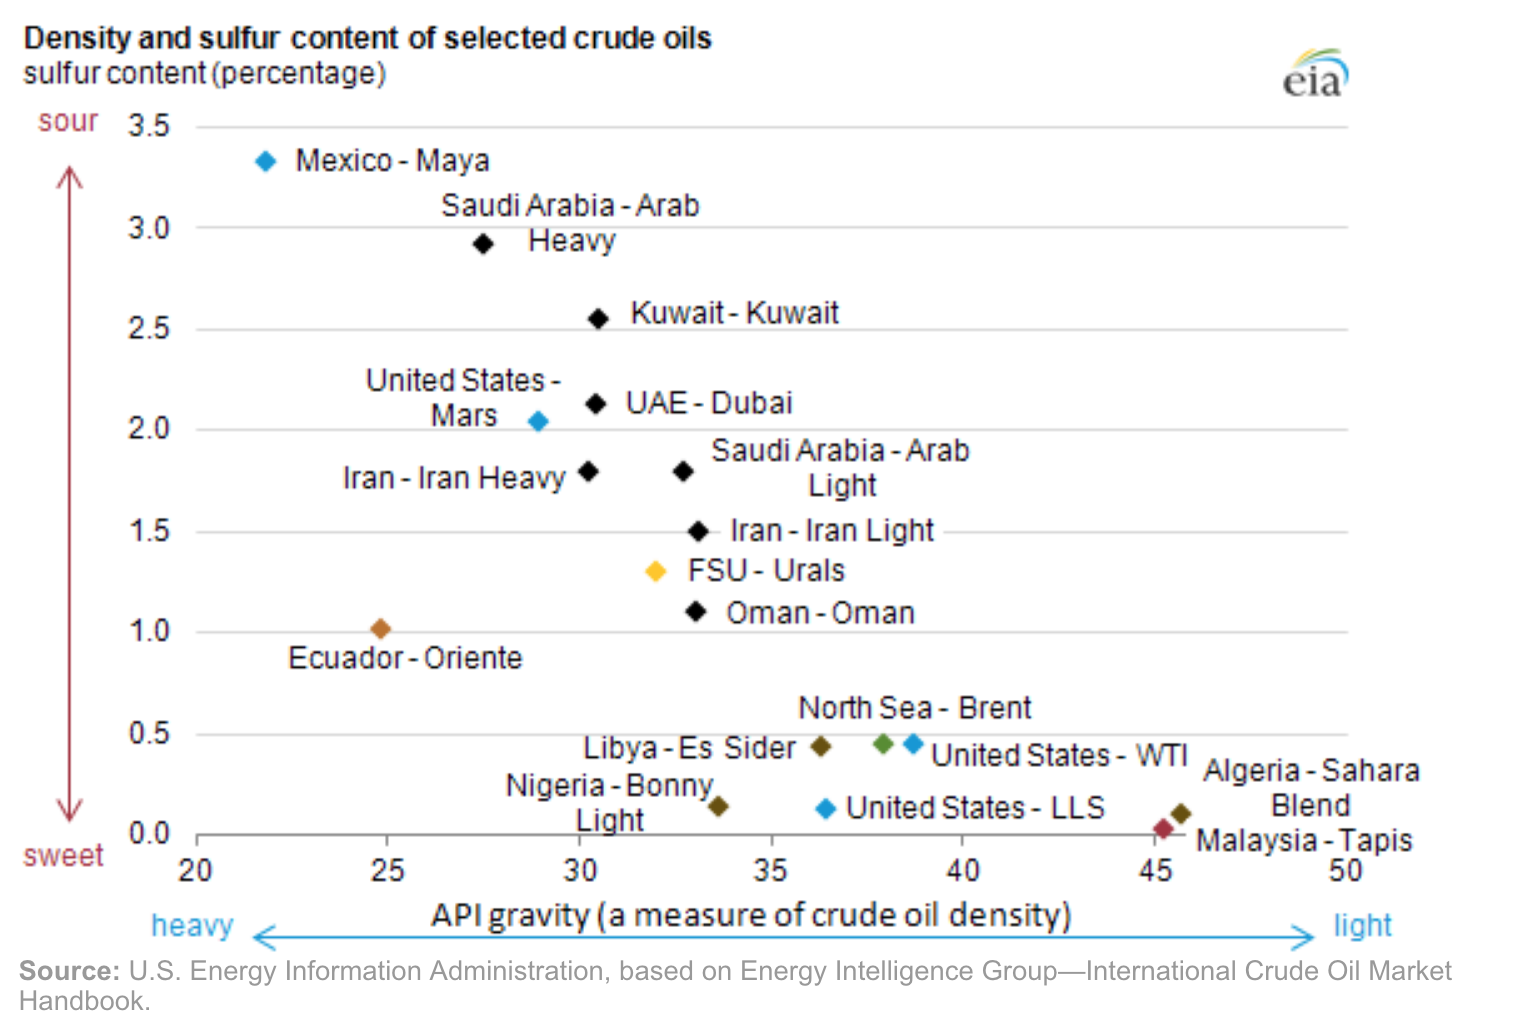
\includegraphics[width=.9\paperwidth]{sweet_and_sour.png}}; \vspace{1cm}
   \vfill
\end{frame}



\begin{frame}{The market has changed since 2014 in many ways}
   \tikz [remember picture,overlay]
    \node[yshift=-.75cm,xshift=0cm] at (current page.center)
        {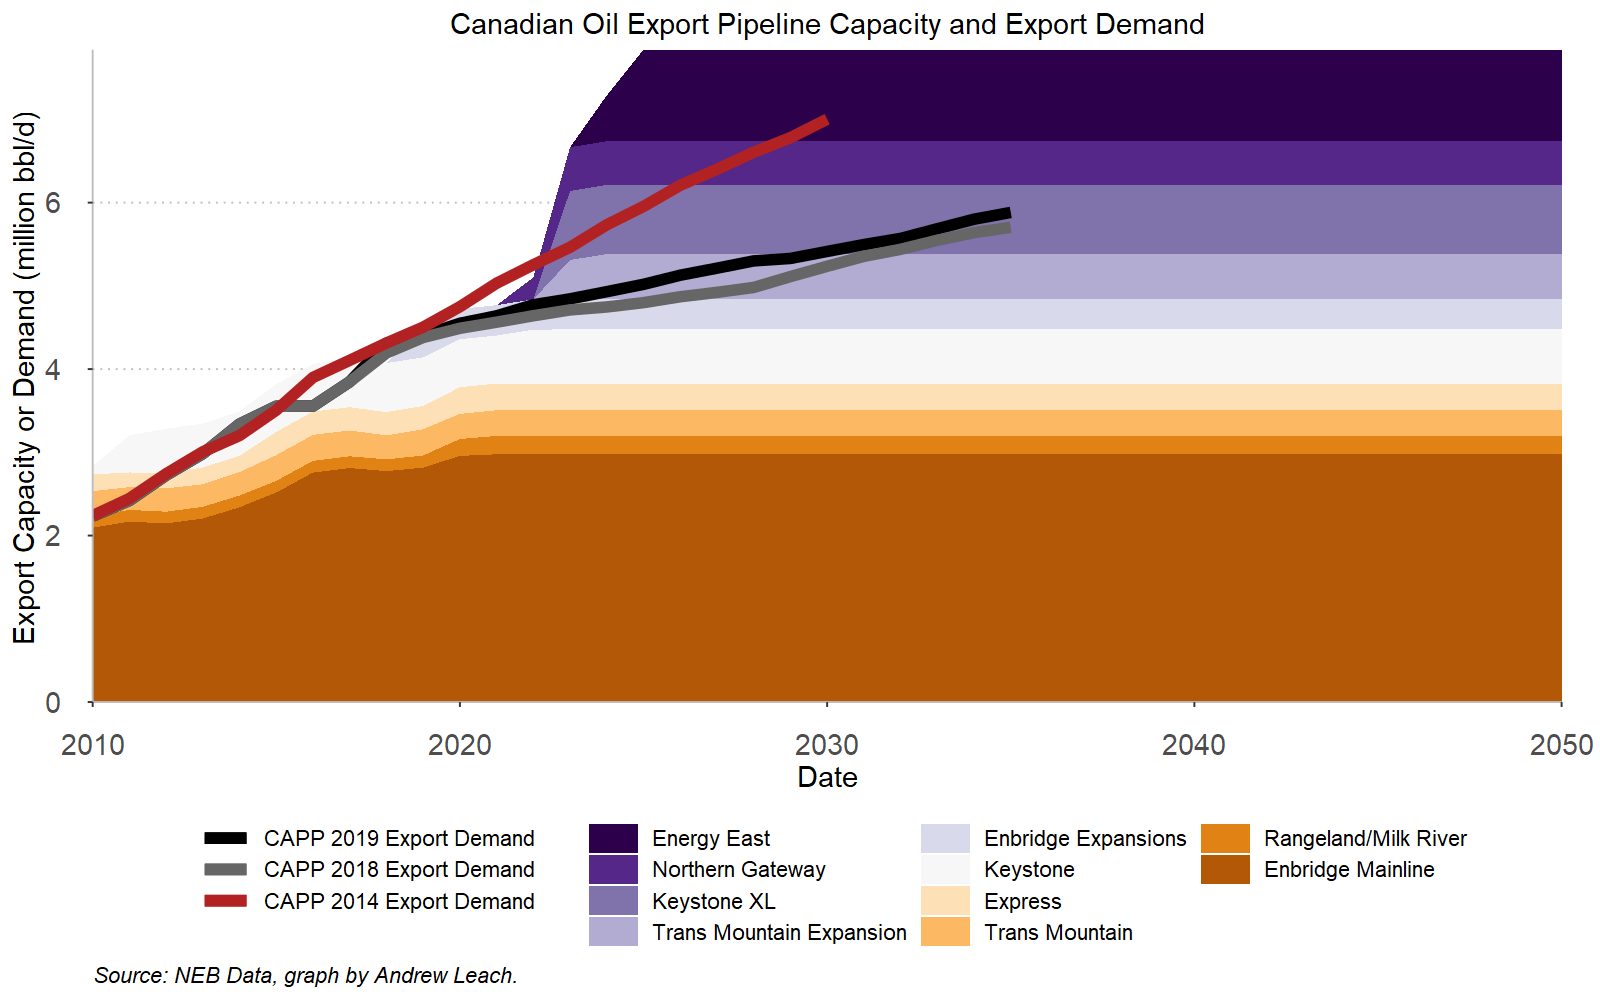
\includegraphics[width=.9\paperwidth]{../../pipe_capacity_new.png}}; \vspace{1cm}
   \vfill
\end{frame}

\begin{frame}{We are short pipe capacity}
   \tikz [remember picture,overlay]
    \node[yshift=-.75cm,xshift=0cm] at (current page.center)
        {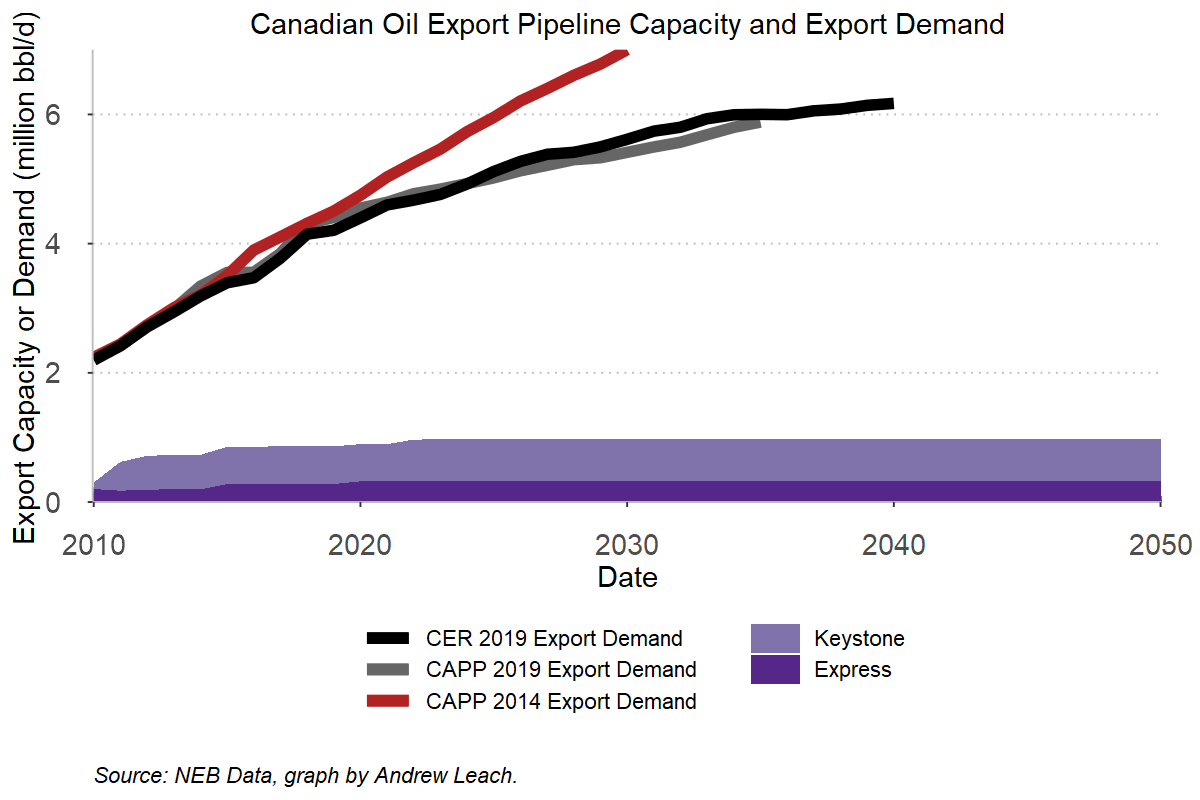
\includegraphics[width=.9\paperwidth]{../../pipe_capacity.png}}; \vspace{1cm}
   \vfill
\end{frame}


\begin{frame}{The consequences of too little pipeline capacity are now clear}
   \tikz [remember picture,overlay]
    \node[yshift=-.75cm,xshift=0cm] at (current page.center)
        {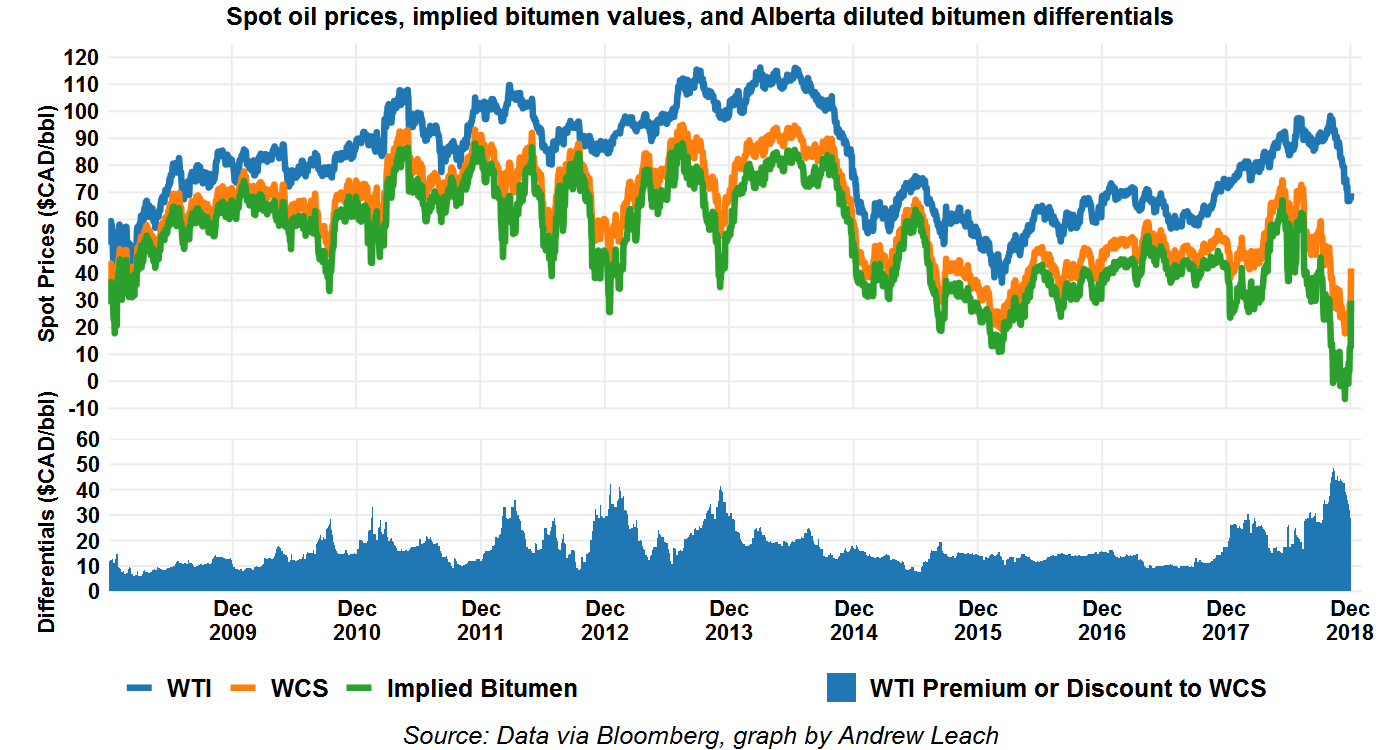
\includegraphics[width=.9\paperwidth]{macleans_2018.png}}; \vspace{1cm}
   \vfill
\end{frame}


\begin{frame}{The consequences of too little pipeline capacity are now clear}
   \tikz [remember picture,overlay]
    \node[yshift=-.75cm,xshift=0cm] at (current page.center)
        {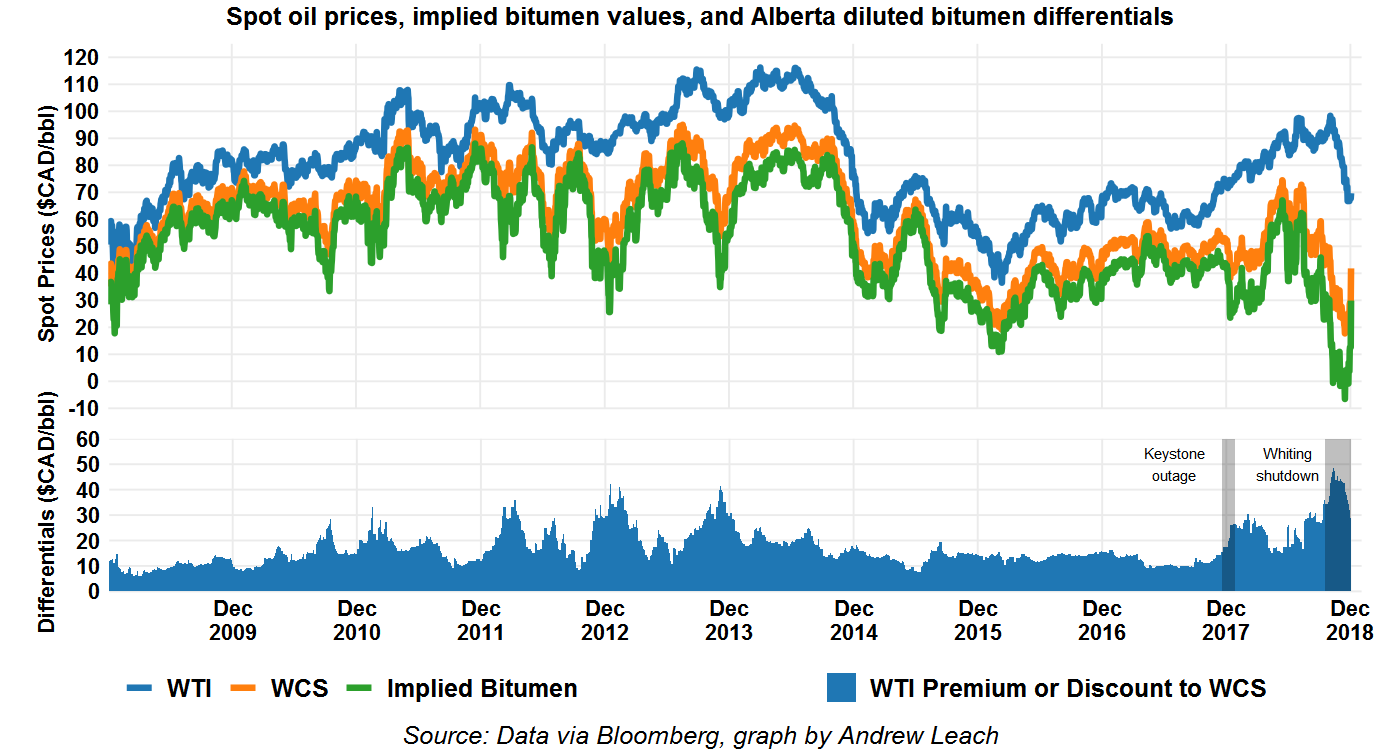
\includegraphics[width=.9\paperwidth]{macleans_2019.png}}; \vspace{1cm}
   \vfill
\end{frame}



\begin{frame}{But it's not just capacity that matters}
\begin{tabular}{p{\linewidth}}
    \centering
    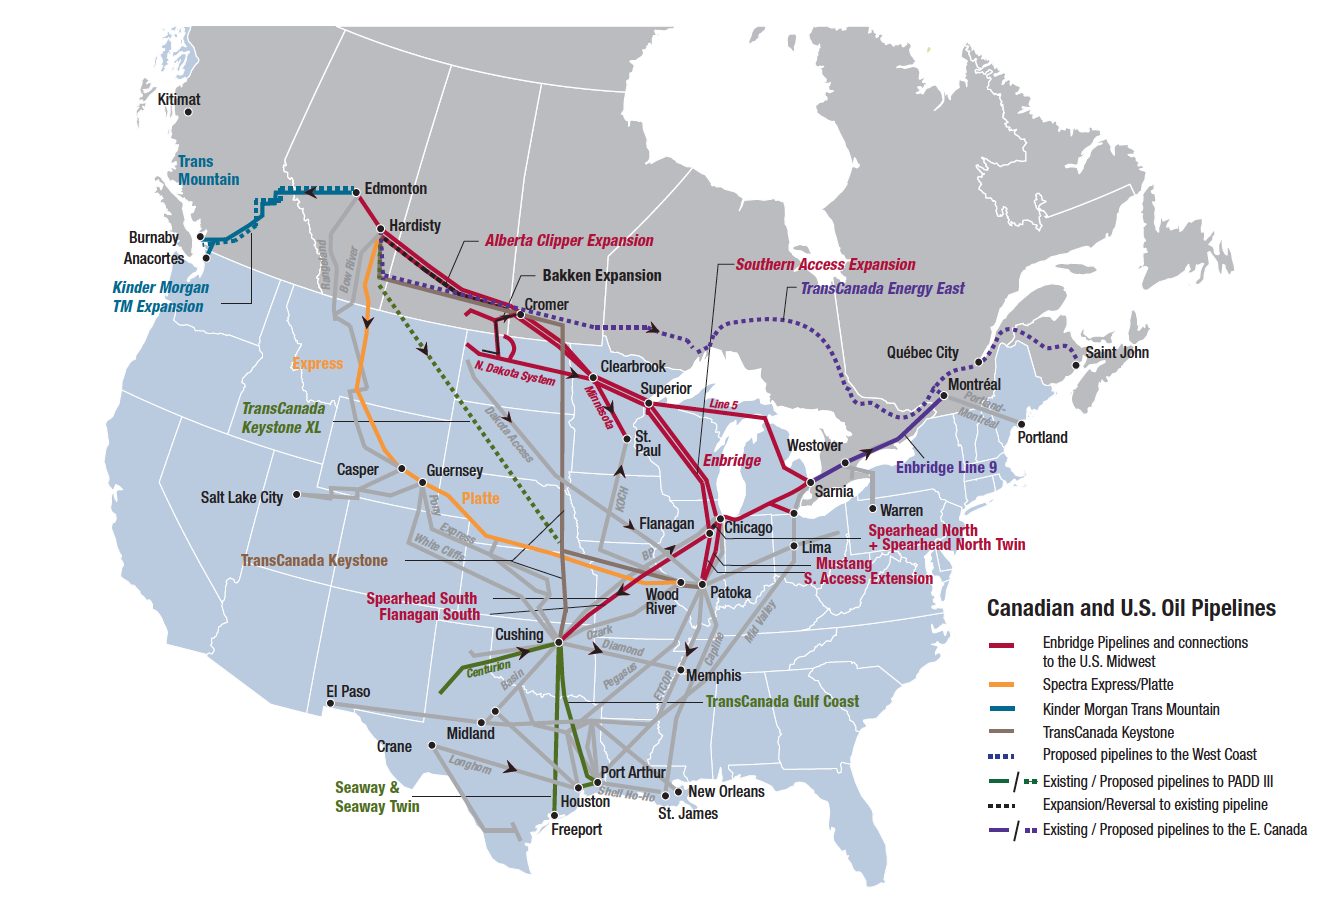
\includegraphics[width=.9\linewidth]{pipeline_map.png} \\[\abovecaptionskip]
  Source: \url{CAPP}
\end{tabular}
\end{frame}

\begin{frame}{A Digression on PADDs}
   \tikz [remember picture,overlay]
    \node[yshift=-.75cm,xshift=0cm] at (current page.center)
        {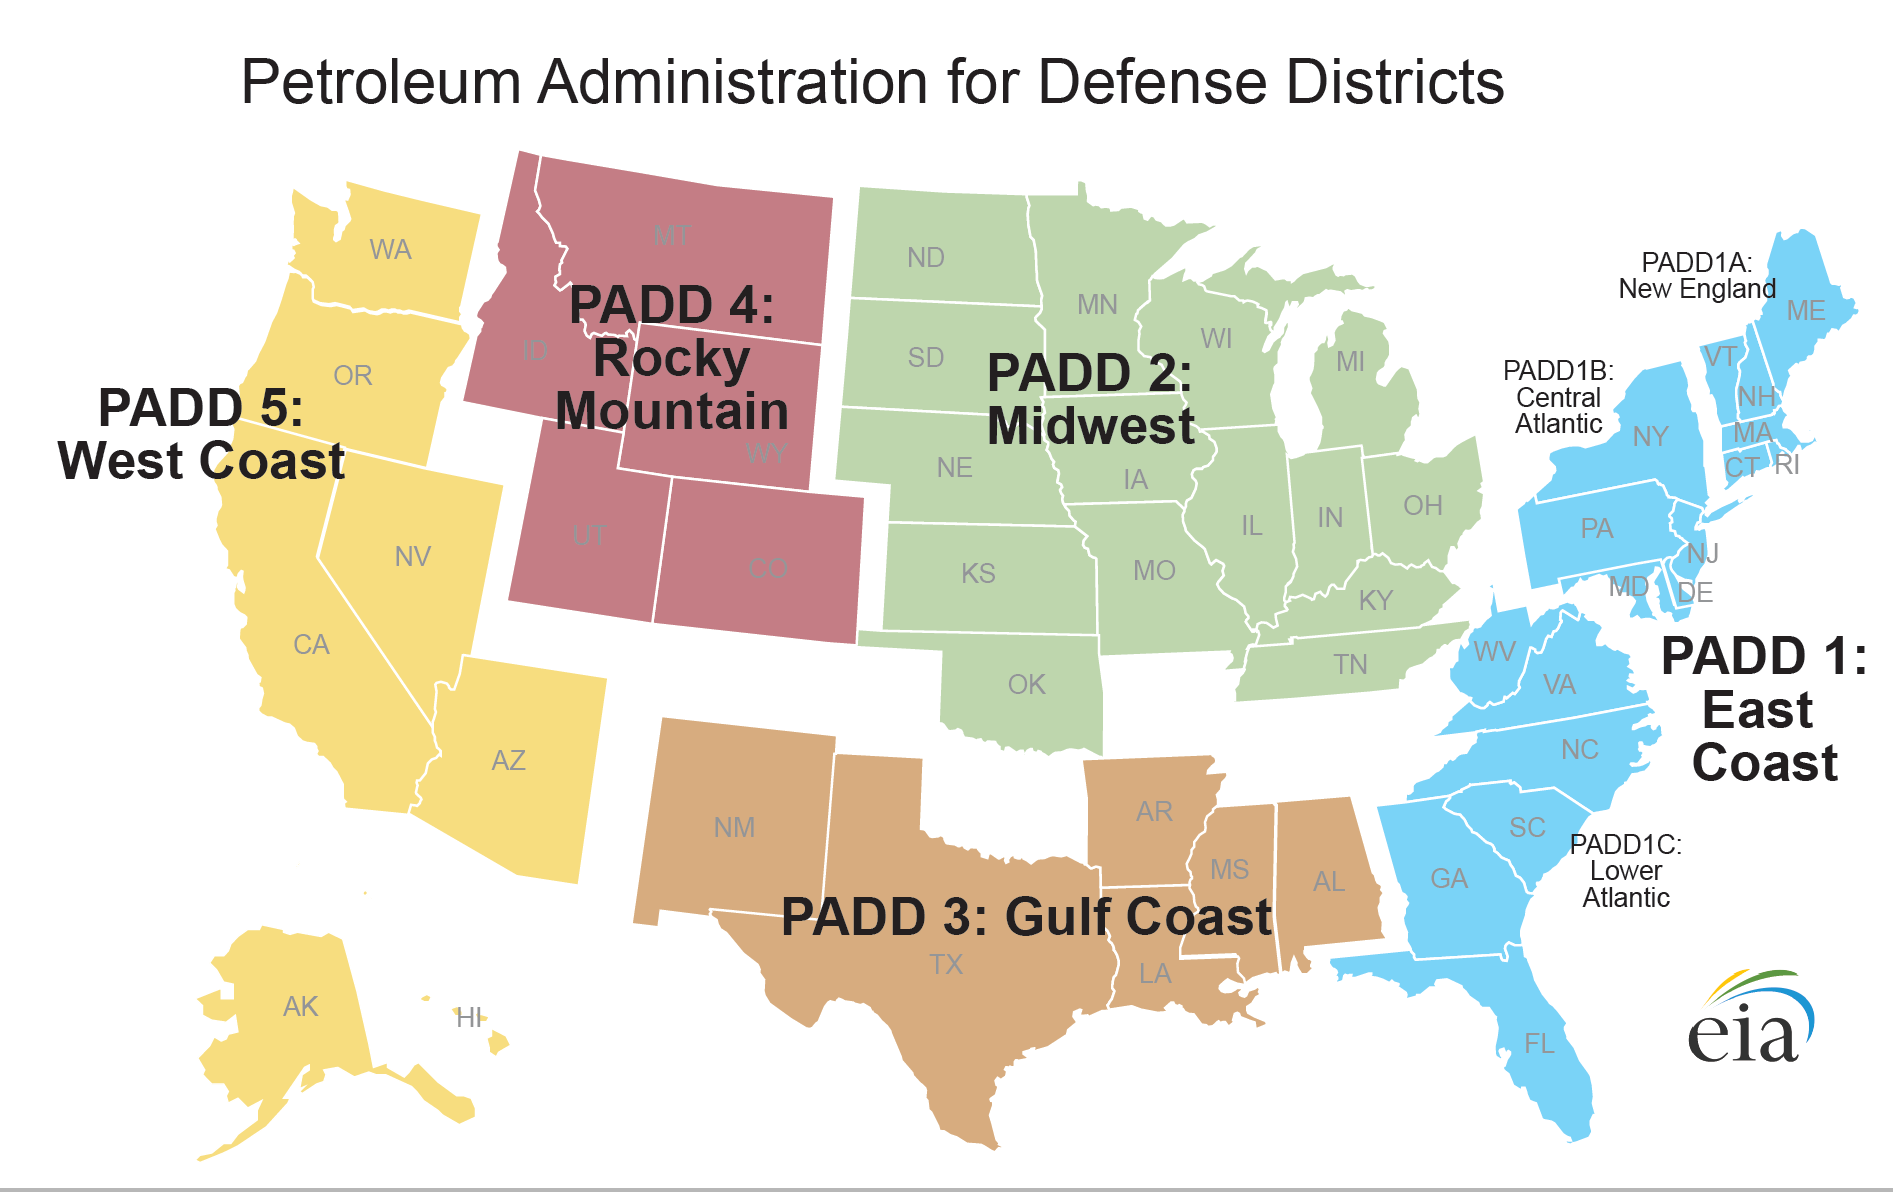
\includegraphics[width=.9\paperwidth]{padd_map.png}}; \vspace{1cm}
   \vfill
\end{frame}


\begin{frame}{Let's not just focus on capacity as markets matter too}
   \tikz [remember picture,overlay]
    \node[yshift=-.75cm,xshift=0cm] at (current page.center)
        {\includegraphics[width=.9\paperwidth]{../../EIA_data_pulls/movements.png}}; \vspace{1cm}
   \vfill
\end{frame}


\begin{frame}{US is producing more, importing less}
   \tikz [remember picture,overlay]
    \node[yshift=-.75cm,xshift=0cm] at (current page.center)
        {\includegraphics[width=.9\paperwidth]{../../EIA_data_pulls/PADD_imports.png}};
         \vspace{1cm}
   \vfill
\end{frame}

\begin{frame}{US is producing more, importing less}
   \tikz [remember picture,overlay]
    \node[yshift=-.75cm,xshift=0cm] at (current page.center)
        {\includegraphics[width=.9\paperwidth]{../../EIA_data_pulls/trade_Crude_Oil.png}};
         \vspace{1cm}
   \vfill
\end{frame}

\begin{frame}{US is producing more, importing less}
   \tikz [remember picture,overlay]
    \node[yshift=-.75cm,xshift=0cm] at (current page.center)
        {\includegraphics[width=.9\paperwidth]{../../EIA_data_pulls/crude_products_trade.png}};
         \vspace{1cm}
   \vfill
\end{frame}



\begin{frame}{Crude flow in the US has shifted: used to be in and north, now it's south and out}
   \tikz [remember picture,overlay]
    \node[yshift=-.75cm,xshift=0cm] at (current page.center)
        {\includegraphics[width=.9\paperwidth]{../../EIA_data_pulls/PADD_exports.png}}; \vspace{1cm}
   \vfill
\end{frame}


\begin{frame}{Complex Capacity Matters to Oil Sands Value}
   \tikz [remember picture,overlay]
    \node[yshift=-.75cm,xshift=0cm] at (current page.center)
        {\includegraphics[width=.9\paperwidth]{../../EIA_data_pulls/refining_capacity.png}}; \vspace{1cm}
   \vfill
\end{frame}


\section{GHG Emissions}

\begin{frame}{Emissions across the economy}
   \tikz [remember picture,overlay]
    \node[yshift=-.75cm,xshift=0cm] at (current page.center)
        {\includegraphics[width=.9\paperwidth]{../../inventory_ghgs.png}}; \vspace{1cm}
   \vfill
\end{frame}


\begin{frame}{Targets, not policies}
   \tikz [remember picture,overlay]
    \node[yshift=-.75cm,xshift=0cm] at (current page.center)
        {\includegraphics[width=.9\paperwidth]{../../emissions_and_targets.png}}; \vspace{1cm}
   \vfill
\end{frame}

\begin{frame}{The Global Challenge is Steep}
   \tikz [remember picture,overlay]
    \node[yshift=-.75cm,xshift=0cm] at (current page.center)
        {\includegraphics[width=.9\paperwidth]{../../emissions_gap.png}}; \vspace{1cm}
   \vfill
\end{frame}


\begin{frame}{The Challenge Ahead for Oil Sands}
   \tikz [remember picture,overlay]
    \node[yshift=-.75cm,xshift=0cm] at (current page.center)
        {\includegraphics[width=.9\paperwidth]{../../inventory_ghgs.png}}; \vspace{1cm}
   \vfill
\end{frame}


\begin{frame}{The Challenge Ahead for Oil Sands}
   \tikz [remember picture,overlay]
    \node[yshift=-.75cm,xshift=0cm] at (current page.center)
        {\includegraphics[width=.9\paperwidth]{../../oil_sands_sector_ghgs.png}}; \vspace{1cm}
   \vfill
\end{frame}

\begin{frame}{The Challenge Ahead for Oil Sands}
   \tikz [remember picture,overlay]
    \node[yshift=-.75cm,xshift=0cm] at (current page.center)
        {\includegraphics[width=.9\paperwidth]{../../oil_sands_emissions_and_targets.png}}; \vspace{1cm}
   \vfill
\end{frame}

\section{Bill C-69 and Climate Tests}

\begin{frame}{What does C-69 really do?}
\begin{itemize}
\setlength\itemsep{.5em}
\item Changes the rules for major projects with respect to impact assessment;
\item Introduces the Canadian Energy Regulator (CER) which will replace the regulatory functions of the NEB;
\item Updates both impact assessment and regulatory functions to include a climate change test;
\item Makes everyone REALLY nervous.
\end{itemize}

\vfill
\end{frame}


\begin{frame}{A digression on climate change - how much insurance do you want to buy?}
   \tikz [remember picture,overlay]
    \node[yshift=-.75cm,xshift=0cm] at (current page.center)
        {\includegraphics[width=.9\paperwidth]{../../IIASA/temp_2Cprob_range_ssp2.png}}; \vspace{1cm}
   \vfill
\end{frame}

\begin{frame}{RCP scenarios translate into temperature trajectories}
   \tikz [remember picture,overlay]
    \node[yshift=-.75cm,xshift=0cm] at (current page.center)
        {\includegraphics[width=.9\paperwidth]{../../IIASA/temps_median_SSP2.png}}; \vspace{1cm}
   \vfill
\end{frame}


\begin{frame}{Let's name the scenarios to make this easier}
   \tikz [remember picture,overlay]
    \node[yshift=-.75cm,xshift=0cm] at (current page.center)
        {\includegraphics[width=.9\paperwidth]{../../IIASA/temps_median_SSP_names2.png}}; \vspace{1cm}
   \vfill
\end{frame}

\begin{frame}{RCP scenarios translate into emissions trajectories}
   \tikz [remember picture,overlay]
    \node[yshift=-.75cm,xshift=0cm] at (current page.center)
        {\includegraphics[width=.9\paperwidth]{../../IIASA/GHG_ssp2.png}}; \vspace{1cm}
   \vfill
\end{frame}



\begin{frame}{Now, let's narrow this down to a couple of scenarios.}
   \tikz [remember picture,overlay]
    \node[yshift=-.75cm,xshift=0cm] at (current page.center)
        {\includegraphics[width=.9\paperwidth]{../../IIASA/temps_iso_median_names2.png}}; \vspace{1cm}
   \vfill
\end{frame}



\begin{frame}{What do these mean for oil demand?}
   \tikz [remember picture,overlay]
    \node[yshift=-.75cm,xshift=0cm] at (current page.center)
        {\includegraphics[width=.9\paperwidth]{../../IIASA/oil_median_iso_60_SSP2.png}}; \vspace{1cm}
   \vfill
\end{frame}


\begin{frame}{What do these mean for oil demand?}
   \tikz [remember picture,overlay]
    \node[yshift=-.75cm,xshift=0cm] at (current page.center)
        {\includegraphics[width=.9\paperwidth]{../../IIASA/oil_iso_60_SSP2.png}}; \vspace{1cm}
   \vfill
\end{frame}


\begin{frame}{C-69: The Canadian Energy Regulator}
      \small \vspace{-.35cm} When approving a pipeline... \\[-0.5em]
      \begin{aquote}{}
      183(2) The Commission must make its recommendation taking into account in light of among other things, any Indigenous knowledge that has been provided to the
Commission and scientific information and data all considerations that appear to it to be relevant and directly related to the pipeline including:\\[-0.5em]
\begin{itemize}\itemsep 0em
\item[a)]
the environmental effects, including any cumulative
environmental effects;
\item[f)] \textbf{the availability of oil, gas (...) to the pipeline;}
\item[g)] \textbf{the existence of actual or potential markets}
\item[j)]the extent to which the effects of the pipeline hinder
or contribute to the Government of Canada's ability
to meet its environmental obligations and its commitments in respect of climate change;
\item[k)] any relevant assessment referred to in section 92
93 or 95 of the Impact Assessment Act; and
(l) any public interest that the Commission considers
may be affected by the issuance of the certificate or the dismissal of the application.
\end{itemize}
      \end{aquote}

\end{frame}

\section{Conclusion}

\begin{frame}{Conclusion}
\begin{itemize}
\setlength\itemsep{.5em}
\item Oil sands projects will, definitely be more valuable with pipelines than without;
\item Does that mean that global emissions will, definitely, be higher with pipelines than without? No.;
\item Serious global action on climate change will, almost assuredly, mean no further oil sands expansion and (dis)orderly wind-down of the oil sands industry over decades;
\item The good news, again: these are the risks that our oil industry is used to dealing with, as is the NEB/CER process. Let it work - don't tie its hands.
\end{itemize}
\vfill
\end{frame}





\begin{frame}{Contact info}
\begin{center}
Andrew Leach\bigskip \\
School of Business, University of Alberta\bigskip \\
Email: \href{mailto:aleach@ualberta.ca}{andrew.leach@ualberta.ca}\bigskip \\
Twitter: \href{http://twitter.com/andrew_leach}{\url{@andrew_leach}}
\end{center}
\vfill
\end{frame}



\begin{frame}{If not oil sands then what?}
  \tikz [remember picture,overlay]
    \node[yshift=-0.5cm,xshift=0cm] at (current page.center)
        {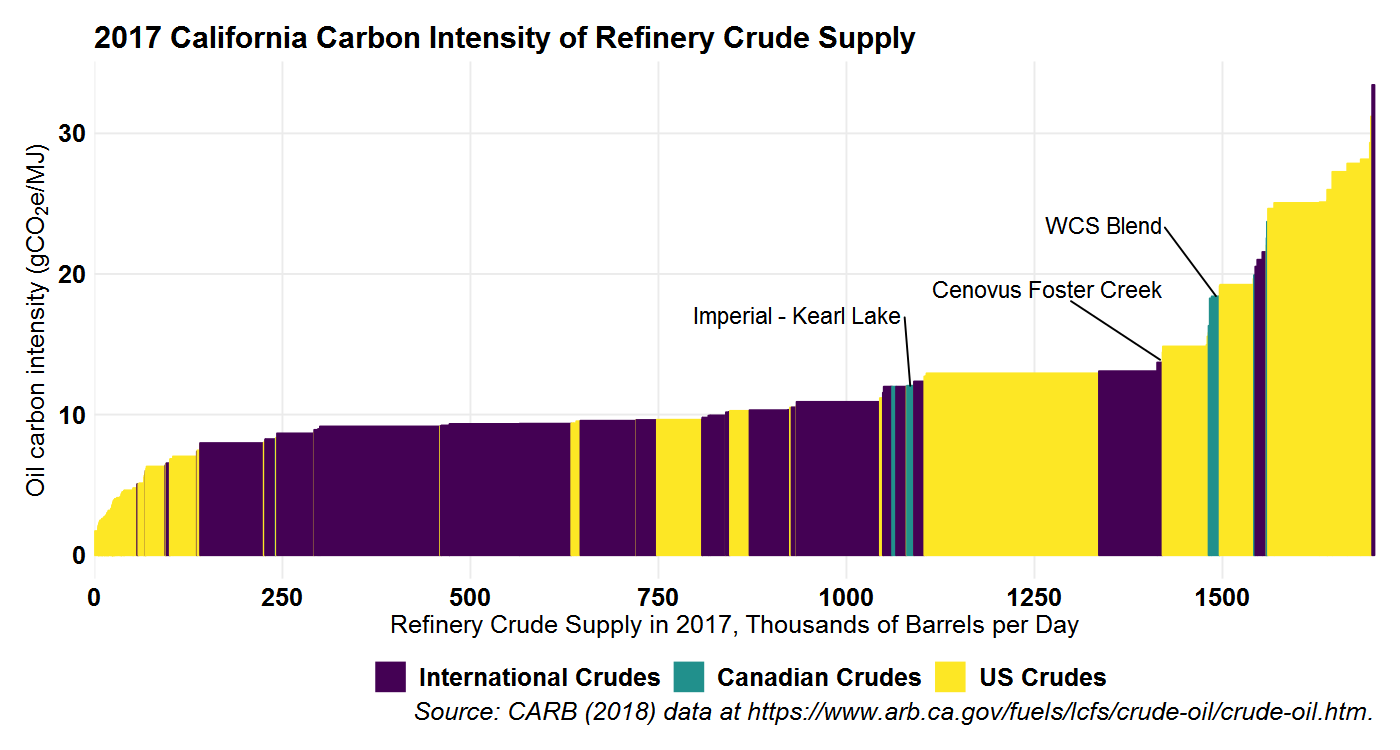
\includegraphics[width=.8\paperwidth]{cali_crude_tab.png}}; \vspace{1cm}
\vfill
\end{frame}

\begin{frame}{If not oil sands then what?}
  \tikz [remember picture,overlay]
    \node[yshift=-0.5cm,xshift=0cm] at (current page.center)
        {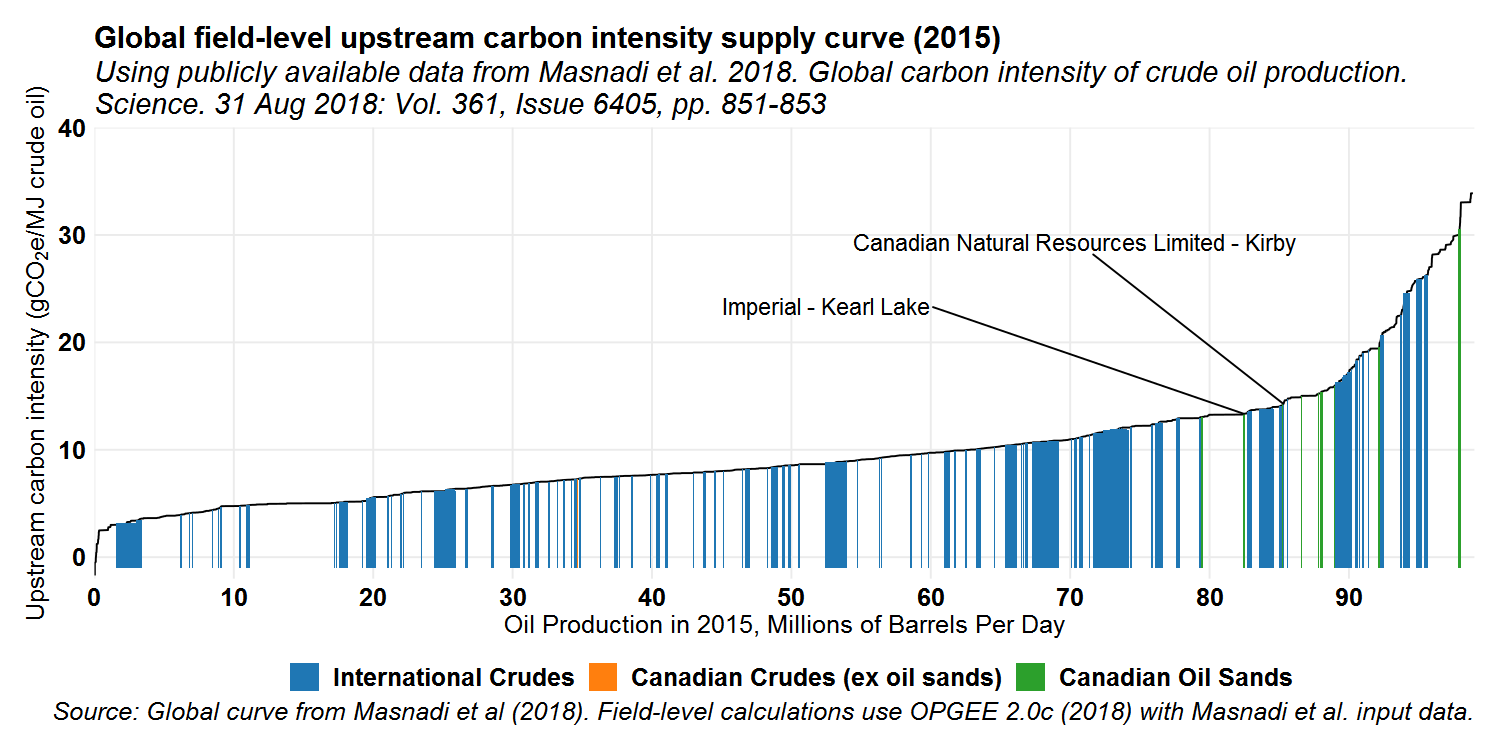
\includegraphics[width=.8\paperwidth]{masnadi.png}}; \vspace{1cm}
\vfill
\end{frame}


\begin{frame}{If not oil sands then what?}
  \tikz [remember picture,overlay]
    \node[yshift=-0.5cm,xshift=0cm] at (current page.center)
        {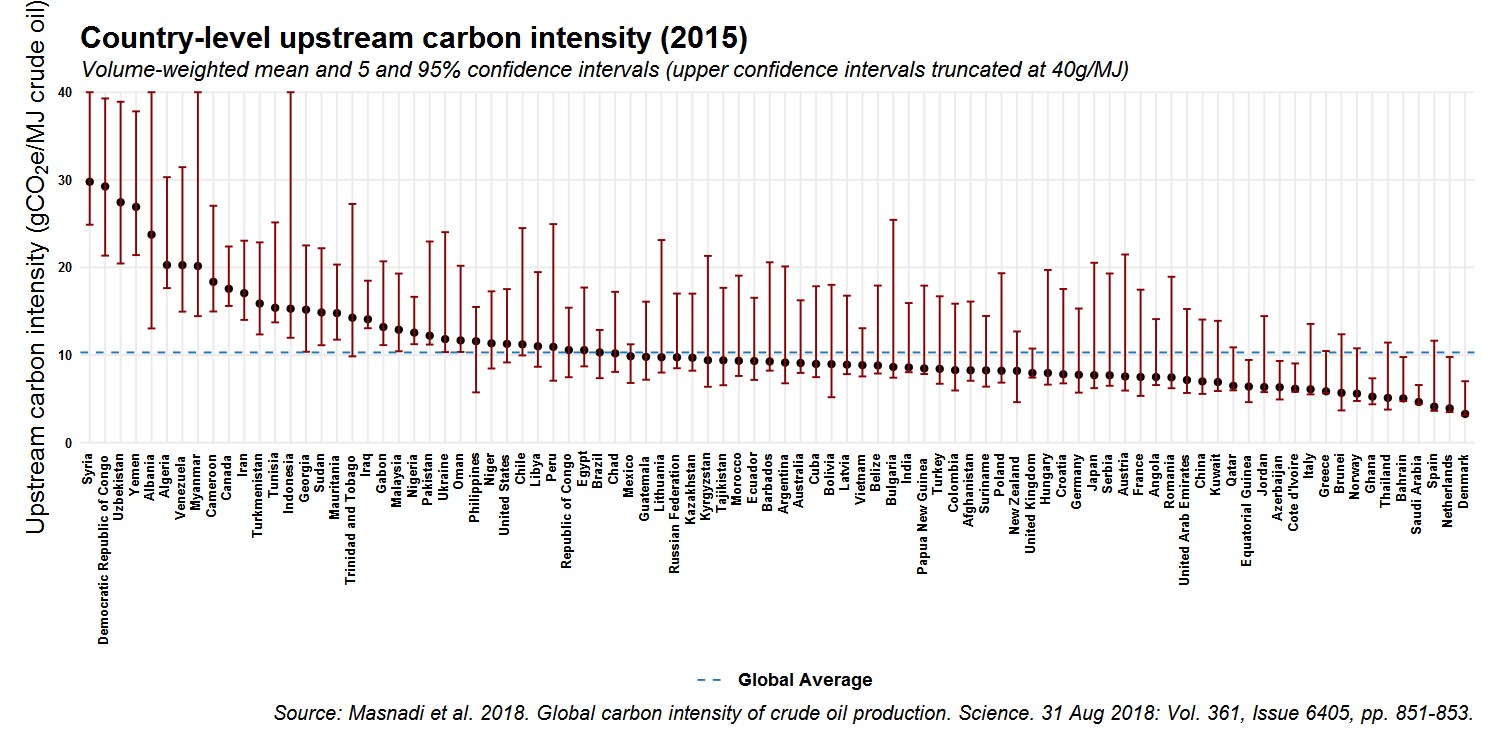
\includegraphics[width=.8\paperwidth]{masnadi_fig_1.png}}; \vspace{1cm}
\vfill
\end{frame}





\end{document} 